\documentclass{article}
\usepackage{amsfonts} % For \mathbb
\usepackage{amsmath} % For align*
\usepackage{enumitem} % For customisable list labels
\usepackage{graphicx} % For images
\usepackage{siunitx} % For units
\graphicspath{{./images/}}

\newcommand{\Span}{\operatorname{Span}}

\title{Advanced Engineering Mathematics Vectors, Matrices, and Vector Calculus by Dennis G. Zill Notes}
\author{Chris Doble}
\date{June 2023}

\begin{document}

\maketitle

\tableofcontents

\section{Vectors}

\subsection{Vectors in 2-Space}

\begin{itemize}
  \item The zero vector can be assigned any direction

  \item The vectors $\textbf{i}$ and $\textbf{j}$ are known as the \textbf{standard basis vectors} for $\mathbb{R}^2$
\end{itemize}

\subsection{Vectors in 3-Space}

\begin{itemize}
  \item In $\mathbb{R}^3$ the octant in which all coordinates are positive is known as the \textbf{first octant}. There is no agreement for naming the other seven octants.
\end{itemize}

\subsection{Dot Product}

\begin{itemize}
  \item The \textbf{dot product} is also known as the \textbf{inner product} or the \textbf{scalar product} and is denoted $\mathbf{a} \cdot \mathbf{b}$

  \item Two non-zero vectors are orthogonal iff their dot product is $0$

  \item The zero vector is considered orthogonal to all vectors

  \item The angles $\alpha$, $\beta$, and $\gamma$ between a vector and the unit vectors $\mathbf{i}$, $\mathbf{j}$, and $\mathbf{k}$, respectively are called the \textbf{direction angles} of the vector

  \item The cosines of a vectors direction angles (the \textbf{direction cosines}) can be calculated as

        \begin{align*}
          \cos \alpha & = \frac{\mathbf{a} \cdot \mathbf{i}}{||\mathbf{a}|| ||\mathbf{i}||} \\
                      & = \frac{a_1}{||\mathbf{a}||}                                        \\
          \cos \beta  & = \frac{\mathbf{a} \cdot \mathbf{j}}{||\mathbf{a}|| ||\mathbf{j}||} \\
                      & = \frac{a_2}{||\mathbf{a}||}                                        \\
          \cos \gamma & = \frac{\mathbf{a} \cdot \mathbf{k}}{||\mathbf{a}|| ||\mathbf{k}||} \\
                      & = \frac{a_3}{||\mathbf{a}||}
        \end{align*}

        Equivalently, these can be calculated as the components of the unit vector $\mathbf{a} / ||\mathbf{a}||$.

  \item To find the component of a vector $\mathbf{a}$ in the direction of a vector $\mathbf{b}$ \[\text{comp}_\mathbf{b} \mathbf{a} = ||\mathbf{a}|| \cos \theta = \frac{\mathbf{a} \cdot \mathbf{b}}{||\mathbf{b}||}\]

  \item To project a vector $\mathbf{a}$ onto a vector $\mathbf{b}$ \[\text{proj}_\mathbf{b} \mathbf{a} = (\text{comp}_\mathbf{b} \mathbf{a}) \frac{\mathbf{b}}{||\mathbf{b}||} = \left( \frac{\mathbf{a} \cdot \mathbf{b}}{\mathbf{b} \cdot \mathbf{b}} \right) \mathbf{b}\]
\end{itemize}

\subsection{Cross Product}

\begin{itemize}
  \item The cross product is only defined in $\mathbb{R}^3$

  \item The \textbf{scalar triple product} of vectors $\mathbf{a}$, $\mathbf{b}$, and $\mathbf{c}$ is defined as \[\mathbf{a} \cdot (\mathbf{b} \times \mathbf{c}) = (\mathbf{a} \times \mathbf{b}) \cdot \mathbf{c} = \begin{vmatrix}
            a_1 & a_2 & a_3 \\
            b_1 & b_2 & b_3 \\
            c_1 & c_2 & c_3
          \end{vmatrix}\]

  \item The area of a parallelogram with sides $\mathbf{a}$ and $\mathbf{b}$ is $||\mathbf{a} \times \mathbf{b}||$

  \item The area of a triangle with sides $\mathbf{a}$ and $\mathbf{b}$ is $\frac{1}{2} ||\mathbf{a} \times \mathbf{b}||$

  \item The volume of a paralleleipied with sides $\mathbf{a}$, $\mathbf{b}$, and $\mathbf{c}$ is $|\mathbf{a} \cdot (\mathbf{b} \times \mathbf{c})|$

  \item $\mathbf{a} \cdot (\mathbf{b} \times \mathbf{c}) = 0$ iff $\mathbf{a}$, $\mathbf{b}$, and $\mathbf{c}$ are coplanar
\end{itemize}

\subsection{Lines and Planes in 3-Space}

\begin{itemize}
  \item There is a unique line between any two points $\mathbf{r_1}$ and $\mathbf{r_2}$ in 3-space. The equation for that line is \[\mathbf{r} = \mathbf{r_1} + t (\mathbf{r_2} - \mathbf{r_1}) = \mathbf{r_1} + t \mathbf{a}\] where $t$ is called a \textbf{parameter}, the nonzero vector $\mathbf{a}$ is called a \textbf{direction vector}, and its components are called \textbf{direction numbers}.

  \item Equating the components of the equation above we find \begin{align*}
          x & = r_1 + t a_1  \\
          y & = r_2 + t a_2  \\
          z & = r_3 + t a_3.
        \end{align*} These are the \textbf{parametric equations} for the line through $\mathbf{r_1}$ and $\mathbf{r_2}$.

  \item By solving the parametric equations for $t$ and equating the results we find the \textbf{symmetric equations} for the line \[t = \frac{x - r_1}{a_1} = \frac{y - r_2}{a_2} = \frac{z - r_3}{a_3}.\]

  \item Given a point $P_1$ and a vector $\mathbf{n}$, there exists only one plane containing $P_1$ with $\mathbf{n}$ normal. The vector from $P_1$ to another point $P$ on that plane will be perpendicular to $\mathbf{n}$, so the equation for the plane is \[\mathbf{n} \cdot (\mathbf{r} - \mathbf{r}_1) = 0\] where $\mathbf{r} = \overrightarrow{O P}$ and $\mathbf{r_1} = \overrightarrow{O P_1}$. If \[\mathbf{n} = a \hat{\mathbf{i}} + b \hat{\mathbf{j}} + c \hat{\mathbf{k}}\] the cartesian form of this equation is \[a (x - x_1) + b (y - y_1) + c (z - z_1) = 0\] and is called the \textbf{point-normal form}.

  \item The graph of any equation $a x + b y + c z + d = 0$, where $a$, $b$, and $c$ are not all zero, is a plane with the normal vector $\mathbf{n} = a \hat{\mathbf{i}} + b \hat{\mathbf{j}} + c \hat{\mathbf{k}}$.

  \item Given three noncollinear points, a normal vector can be found by forming two vectors from two pairs of points and take their cross product.

  \item A line and a plane that aren't parellel intersect at a single point.

  \item Two planes that aren't parallel must intersect in a line.
\end{itemize}

\subsection{Vector Spaces}

\begin{itemize}
  \item The length of a vector is called its \textbf{norm}

  \item The process of multipying a vector by the reciprocal of its norm is called \textbf{normalizing} the vector

  \item Two nonzero vectors $\mathbf{a}$ and $\mathbf{b}$ in $\mathbb{R}^n$ are said to be orthogonal if $\mathbf{a} \cdot \mathbf{b} = 0$
\end{itemize}

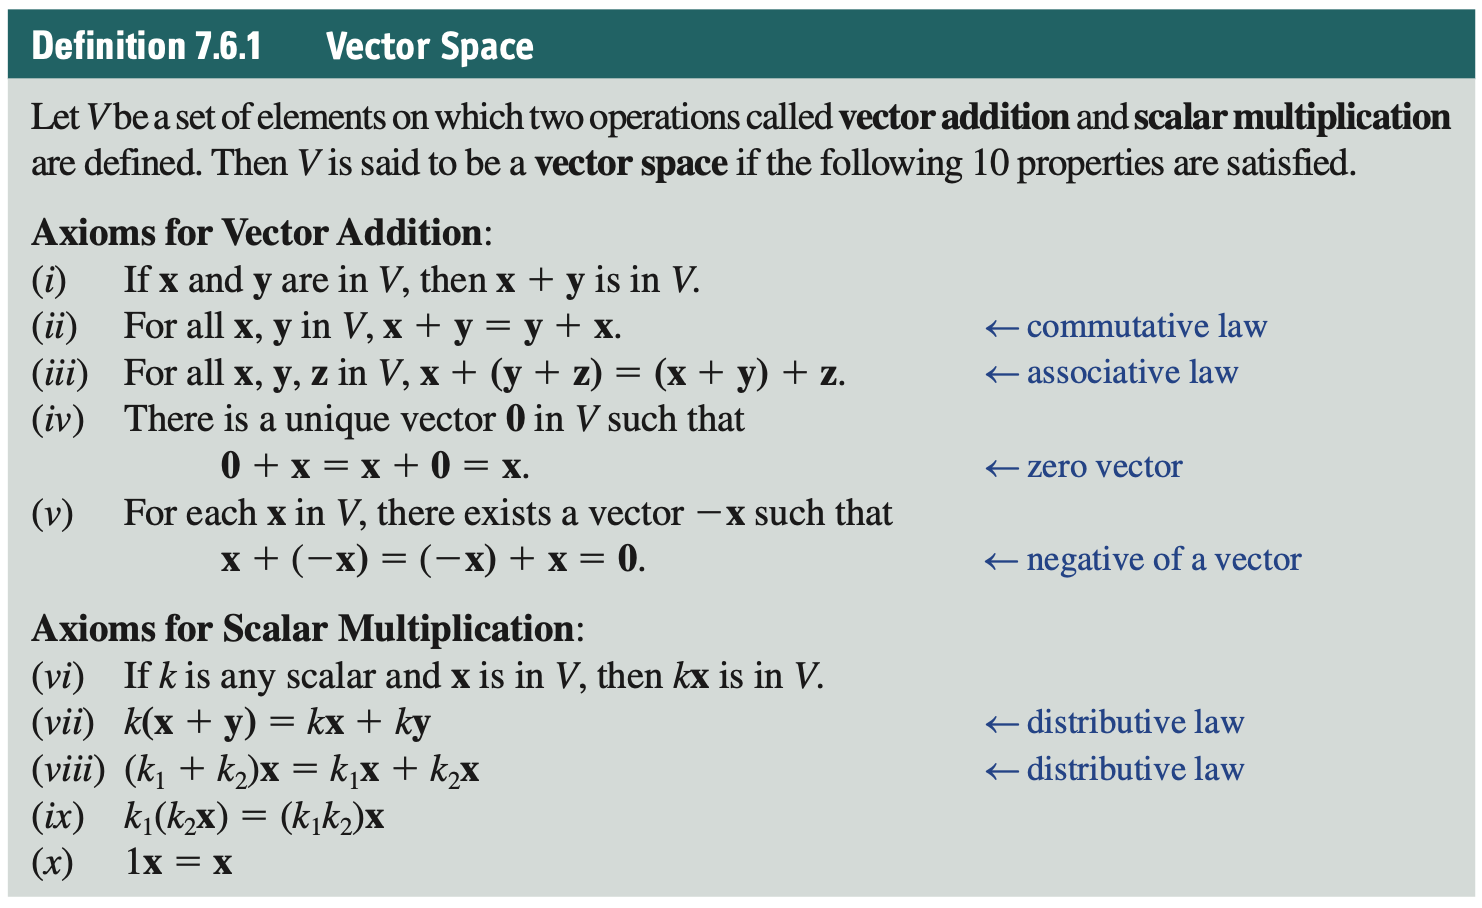
\includegraphics[scale=0.443]{vector-space}

\begin{itemize}
  \item If a subset $W$ of a vector space $V$ is itself a vector space under the operations of vector addition and scalar multiplication defined on $V$, then $W$ is called a \textbf{subspace} of $V$

  \item Every vector space has at least two subspaces: itself and the zero subspace $\{\mathbf{0}\}$

  \item A set of vectors $\{\mathbf{x_1}, \mathbf{x_2}, \ldots, \mathbf{x_n}\}$ is said to be \textbf{linearly independent} if the only constants satisfying the equation \[k_1 \mathbf{x_1} + k_2 \mathbf{x_2} + \cdots + k_n \mathbf{x_n} = \mathbf{0}\] are $k_1 = k_2 = \cdots = k_n = 0$. If the set of vectors is not linearly independent it is said to be \textbf{linearly dependent}.

  \item If a set of vectors $B = \{\mathbf{x}_1, \mathbf{x}_2, \ldots, \mathbf{x}_n\}$ in a vector space $V$ is linearly independent and every vector in $V$ can be expressed as a linear combination of vectors in $B$ then $B$ is said to be a \textbf{basis} for $V$.

  \item The number of vectors in a basis $B$ for a vector space $V$ is said to be the \textbf{dimension} of the space.

  \item If the basis of a vector space contains a finite number of vectors, then the space is \textbf{finite dimensional}; otherwise it is \textbf{infinite dimensional}.

  \item If $S$ denotes any set of vectors $\{\mathbf{x}_1, \mathbf{x}_2, \ldots, \mathbf{x}_n\}$ in a vector space $V$, then the set of all linear combinations of the vectors in $S$ \[c_1 \mathbf{x}_1 + c_2 \mathbf{x}_2 + \cdots + c_n \mathbf{x}_n\] is called the \textbf{span} of the vectors and is denoted $\Span(S)$.

  \item $\Span(S)$ is a subspace of $V$ and is said to be a subspace spanned by its vectors $\mathbf{x}_1, \mathbf{x}_2, \ldots, \mathbf{x}_n$.

  \item If $V = \Span(S)$ then $S$ is said to be a \textbf{spanning set} for the vector space $V$ or that $S$ \textbf{spans} $V$.
\end{itemize}

\subsection{Gram–Schmidt Orthogonalization Process}

\begin{itemize}
  \item An \textbf{orthonormal basis} is a basis whose vectors are mutually orthogonal and are unit vectors.

  \item If $B = \{\mathbf{w}_1, \mathbf{w}_2, \ldots, \mathbf{w}_n\}$ is an orthonormal basis for $\mathbb{R}^n$ then an arbitrary vector $\mathbf{u}$ can be expressed as \[\mathbf{u} = (\mathbf{u} \cdot \mathbf{w}_1) \mathbf{w}_1 + (\mathbf{u} \cdot \mathbf{w}_2) \mathbf{w}_2 + \cdots + (\mathbf{u} \cdot \mathbf{w}_n) \mathbf{w}_n\]

  \item The \textbf{Gram-Schmidt Orthogonalization Process} is a process for converting any basis of a vector space into an orthonormal basis. First the basis vectors are made orthogonal to each other, then they are normalized. More specifically, to convert a basis $B = \{\mathbf{u}_1, \mathbf{u}_2, \ldots, \mathbf{u}_n\}$ into an orthogonal basis $B' = \{\mathbf{v}_1, \mathbf{v}_2, \ldots, \mathbf{v}_n\}$

        \begin{enumerate}
          \item Let $\mathbf{v}_1 = \mathbf{u}_1$

          \item Let $\mathbf{v}_2 = \mathbf{u}_2 - \text{proj}_{\mathbf{v}_1} \mathbf{u}_2$

          \item \ldots

          \item Let $\mathbf{v}_n = \mathbf{u}_n - \text{proj}_{\mathbf{v}_1} \mathbf{u}_n - \text{proj}_{\mathbf{v}_2} \mathbf{u}_n - \cdots - \text{proj}_{\mathbf{v}_{n - 1}} \mathbf{u}_n$
        \end{enumerate}

        and to convert $B'$ into an orthonormal basis $B'' = \{\mathbf{w}_1, \mathbf{w}_2, \ldots, \mathbf{w}_n\}$, normalize each $\mathbf{v}_i$, $i = 1, 2, \ldots, n$.
\end{itemize}

\section{Matrices}

\subsection{Matrix Algebra}

\begin{itemize}
  \item Vectors can be written as horizontal or vertical arrays of numbers

  \item A \textbf{matrix} is any rectangular array of numbers or functions \[\begin{pmatrix}
            a_{11} & a_{12} & \cdots & a_{1n} \\
            a_{21} & a_{22} & \cdots & a_{2n} \\
            \vdots &        &        & \vdots \\
            a_{m1} & a_{m2} & \cdots & a_{mn}
          \end{pmatrix}\]

  \item The numbers or functions in the array are called the \textbf{elements} or \textbf{entries} of the matrix

  \item If a matrix has $m$ rows and $n$ columns we say that its \textbf{size} is $m$ by $n$ or $m \times n$

  \item An $n \times n$ matrix is called a \textbf{square} matrix of \textbf{order $n$}

  \item The entry in the $i$th row and the $j$th column of an $m \times n$ matrix $\mathbf{A}$ is written $a_{ij}$

  \item An $m \times 1$ matrix \[\begin{pmatrix}
            a_1    \\
            a_2    \\
            \vdots \\
            a_n
          \end{pmatrix}\] is called a \textbf{column vector}

  \item A $1 \times n$ matrix \[\begin{pmatrix}
            a_1 & a_2 & \cdots & a_n
          \end{pmatrix}\] is called a \textbf{row vector}
\end{itemize}

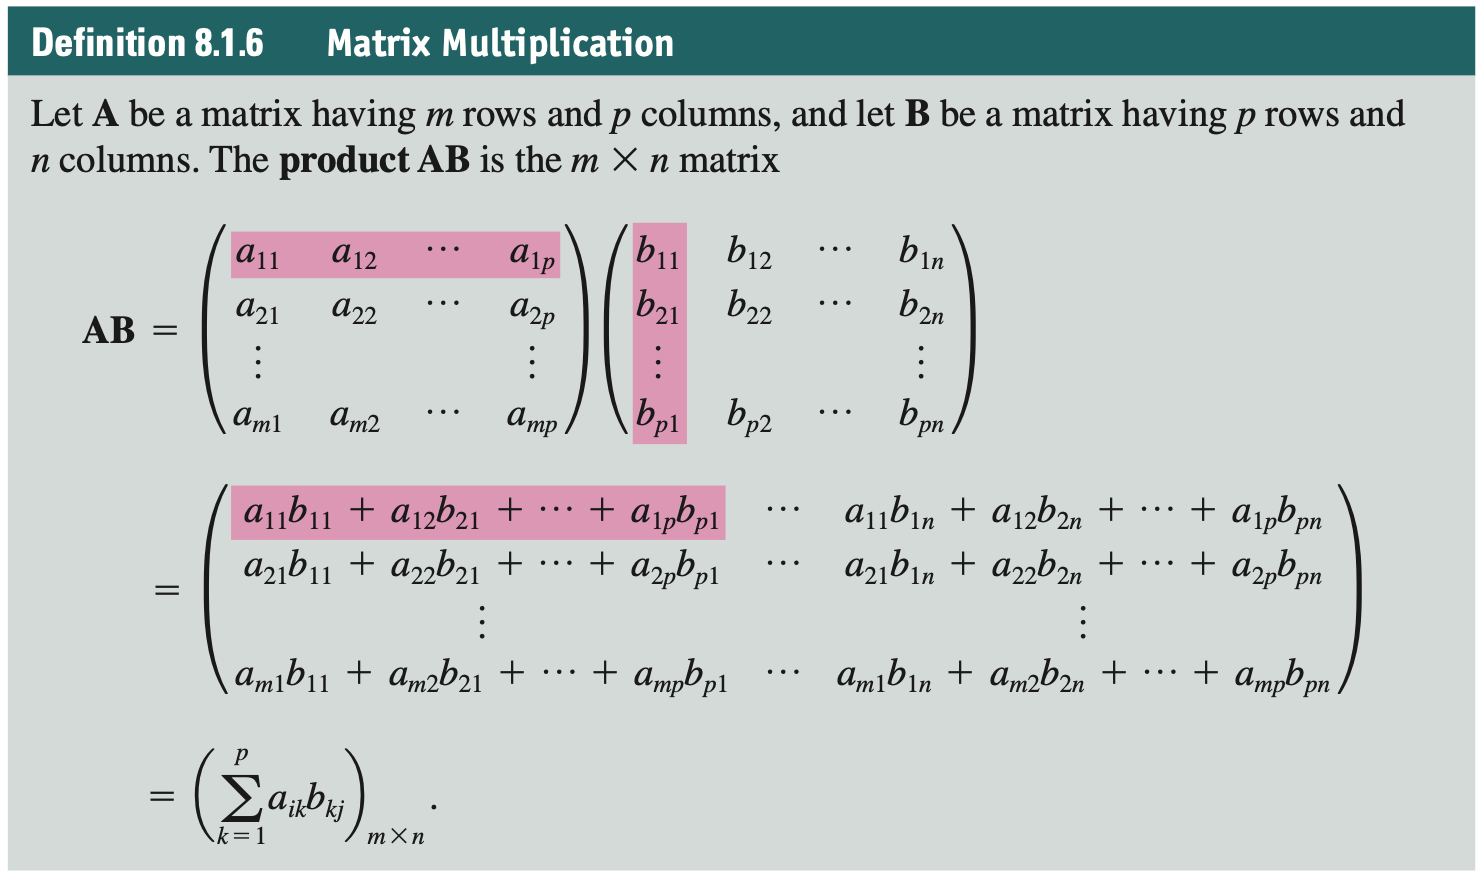
\includegraphics[scale=0.443]{matrix-multiplication}

\begin{itemize}
  \item Matrix multiplication is associative, i.e. $\mathbf{A} (\mathbf{B} \mathbf{C}) = (\mathbf{A} \mathbf{B}) \mathbf{C}$

  \item Matrix multiplication is distributive, i.e. $\mathbf{A} (\mathbf{B} + \mathbf{C}) = \mathbf{A} \mathbf{B} + \mathbf{A} \mathbf{C}$ and $(\mathbf{B} + \mathbf{C}) \mathbf{A} = \mathbf{B} \mathbf{A} + \mathbf{C} \mathbf{A}$

  \item The \textbf{transpose} of an $m \times n$ matrix $\mathbf{A}$ is an $n \times m$ matrix $\mathbf{A}^T$ \[\begin{pmatrix}
            a_{11} & a_{21} & \cdots & a_{m1} \\
            a_{12} & a_{22} & \cdots & a_{m2} \\
            \vdots &        &        & \vdots \\
            a_{1n} & a_{2n} & \cdots & a_{mn}
          \end{pmatrix}\] i.e. the matrix is flipped along the main diagonal
\end{itemize}

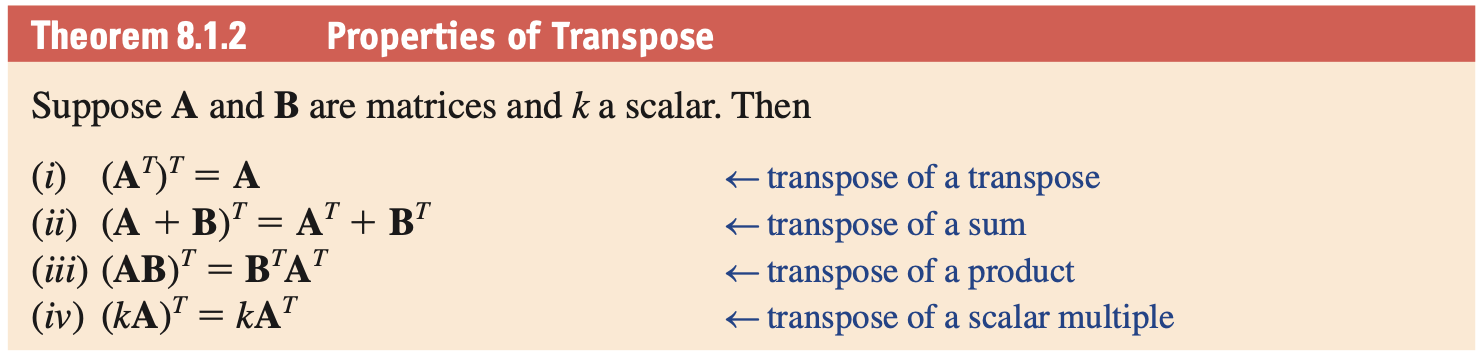
\includegraphics[scale=0.443]{transpose-properties}

\begin{itemize}
  \item A matrix that consists of all zero entries is called a \textbf{zero matrix}

  \item A square matrix is said to be a \textbf{triangular matrix} if all of its entries above or below the main diagonal are zeroes. More specifically they are called \textbf{lower triangular} and \textbf{upper triangular} matrices, respectively.

  \item A square matrix is called a \textbf{diagonal matrix} if all entries not on the main diagonal are 0.

  \item A square matrix whose entries on the main diagonal are all equal is called a \textbf{scalar matrix}

  \item A square matrix that has the property $\mathbf{A} = \mathbf{A}^T$ is called a \textbf{symmetric matrix}
\end{itemize}

\end{document}